\section{Barrel Electromagnetic Calorimeter (BEMC)}

	Τα καλορίμετρα αποτελεούν καταστρεπτικούς ανιχνευτές, δηλαδή επιτελούν τις διάφορες διαδικασίες ανίχνευσης εξαναγκάζοντας τα σωματίδια να εναποθέσουν την ενέργειά τους στο υλικό και εν τέλει να σταματήσουν. Άρα στην συνέχεια τα σωματίδια δεν θα είναι διαθέσιμα για περεταίρω μετρήσεις, όπως συμβαίνει για παράδειγμα όταν διέρχονται από έναν TPC, και γι' αυτό τα καλορίμετρα τοποθετούνται συνήθως στα εξωτερικά στώματα των ανιχνευτών. 
	
	Ο STAR έχει δύο ηλεκτρομαγνητικά καλορίμετρα, το Barrel Electromagnetic Calorimeter (BEMC) και το Endcap Electromagnetic Calorimeter (EEMC). Αυτά βασίζονται στο φαινόμενο του ηλεκτρομαγνητικού καταιγισμού, ο οποίος προκαλείται όταν ένα υψηλής ενέργειας ηλεκτρόνιο ή φωτόνιο προσπίπτει σε πυκνό υλικό. Πιό συγκεκριμένα, όταν ένα ηλεκρόνιο ταξιδέψει σε ένα υλικό για μήκος ίσο με το radiaition length $X_0$, τότε θα ακτινοβολήσει σίγουρα ένα φωτόνιο Bremstralhung, ενώ ένα ενεργητικό φωτόνιο έχει περίπου 64\% πιθανότητα να κάνει διδυμη η γέννηση και να παραχθεί ζεύγος $e^-e^+$. Συνεπώς σε $X_0$ έχουμε διπλασιασμό των σωματιδίων και μετά από $\Delta x = t\cdot X_0$ θα έχουμε $n(t) = 2^t$ σωματίδια. 
	
	Η ανάπτυξη του καταιγισμού οδηγεί σε αύξηση του αριθμού δευτερογενών ηλεκτρονίων και φωτονίων επομένως στην μείωση της ενέργειας του καθε νέου σωματιδίου. Για παράδειγμα, αν η ενέργεια του αρχικού σωματιδίου είναι $E_0$, τότε στο πρώτο $X_0$ κάθε νέο σωματίδιο αποκτά ενέργεια $E_0/2$, άρα μετά από $\Delta x = t\cdot X_0$ κάθε σωματίδιο έχει ενέργεια $E(t) = E_0\cdot 2^t$.
	
	Γίνεται αισθητό πως καθώς μειώνεται η ενέργεια των σωματιδίων αυτά δεν θα χάνουν ενέργεια κυρίως με Bremstahlung αν είναι ηλεκτρόνια και δεν θα μπορούν να κάνουν δίδυμη γέννηση αν είναι φωτόνια. Συνεπώς είναι λογικό να υπάρχει μία ενέργεια κάτω από την οποία να μην είναι δυνατή η συνέχιση του καταιγισμού. 
	Αυτή η ενέργεια είναι η κρίσιμη ενέργεια, δηλαδή αυτή στην οποία οι απώλειες του αρχικού ηλεκτρονίου από Bremstrahlung και ιονισμό του υλικού είναι ίσες. Από εκεί και πέρα η ενέργεια των εναπομείναντων σωματιδίων του καταιγισμού χάνεται μέσω ιονισμών και διεγέρσεων του υλικού που διασχίζουν.
	
	Άρα η συνθήκη τερματισμού του Ηλεκτρομαγνητικού Καταιγισμού είναι 
		\begin{equation*}\label{eq3.3}
			E(t_{max}) = E_c \numberthis
		\end{equation*}
	Από την οποία προκύπτει και ο μέγιστος αριθμός γενεών σωματιδίων 
		\begin{equation}\label{eq3.4}
			t_{max} = \frac{lN(E_0/E_c)}{ln(2)}
		\end{equation}
	Ένας τυπικός αριθμός γενεών είναι 20-25 άρα θέλουμε ένα υλικό 20-25$X_0$ προκειμένου να παγιδεύσουμε πλήρως τον Ηλεκτρομαγνητικό Καταιγισμό του αρχικού σωατιδίου άρα και όλη του την ενέργεια.
	
	 Τα παραπάνω ήταν σχετικά με την διαμήκη συμπεριφορά του Καταιγισμού της οποίας τυπικό μήκος είναι το μήκος ακτινοβολίας $X_0$. Η εγκάρσια συμπεριφορά του καθορίζεται από τις πολλαπλές σκεδάσεις Coulomb με τους πυρήνες του υλικού που έχουμε επιλέξει και το χαρακτηριστικό της μήκος είναι η ακτίνα Moliere η οποία ορίζεται ως 
	 \begin{align}\label{eq3.5}
	 	R_M = \frac{(charact. energy)\times X_0}{E_c}
	 \end{align}
	όπου η χαρακτηριστική ενέργεια είναι $\simeq21MeV$. αν είχαμε έναν κύλινδρο απείρου μήκους και ακτίνας $R_M$, τότε αυτός θα περιείχε το 90\% της ενέργειας του καταιγισμού, ενώ αν η ακτίνα του ήταν $2R_M$ θα περιείχε το 95\%.
	
	
	Υπάρχουν καλορίμετρα διαφόρων ειδών που ποικίλουν ως προς τα χαρακτηριστικά  και την διακριτική ικανότητά τους και επιλέγονται ανάλογα με τις ανάγκες του εκάστοτε πειράματος. Το BEMC του STAR, είναι ένα Scintillating Sampling Calorimeter με Μόλυβδο, το οποίο ήταν μία βολική, ευέλικτη και οικονομική επιλογή για να καλύψει τους περιορισμούς που επιβάλλει η γεωμετρία του STAR, όπου θα πρέπει να τοποθετηθεί σε έναν κλειστό χώρο ενδιάμεσα από άλλους ανιχνευτές, συστήματα και εντός μαγνητικού πεδίου. 
	
%	\begin{figure}[h!]
%			\centering 
%			\includegraphics[scale=0.5]{STAR_Detectors/Detectors_Cross_Section.png}
%			\caption{Τομές του STAR όπου φαίνεται η θέση του BEMC}
%			\label{fig3.11}
%		\end{figure}
			
			\begin{figure}[h!]
				\centering
				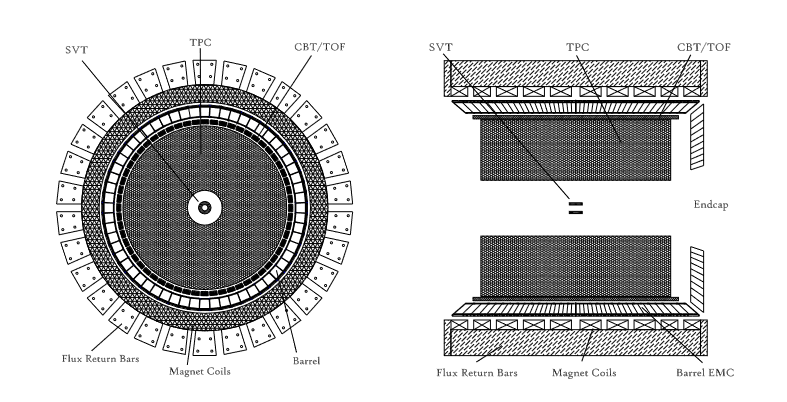
\includegraphics[scale=0.4]{STAR_Detectors/Detectos_Cross_Section}
				\caption{Τομές του STAR όπου φαίνεται η θέση του BEMC}
				\label{fig3.11}
			\end{figure}
	
	
	Ο στόχος του είναι η μελέτη διαδικασιών με υψηλή κάθετη ορμή $p_T$, όπως πίδακες, βαρέα κουάρκ και να παρέχει μεγάλη γεωμετρικη αποδοχή σε πρωτόνια, ηλεκτρόνια, $\pi^0$ και $\eta$ μεσόνια προερχόμενα από κρούσεις πολωμένων πρωτονίων και Au-Au. 
	Καλύπτει μία γεωμετρική περιοχή $60m^2$ για pseudorapidity $|\eta|<1$.
	Για την επίτευξη των στόχων θα πρέπει να είναι σε θέση να εγκλωβίσει ενέργεια καταιγισμού 60GeV και γι' αυτό έχει ακτίνα 20$X_0$.
	
	Ο BEMC κατασκευάζεται από μικρά τμήματα μολύβδου και πλαστικού σπινθηριστή για να είναι ευκολότερη η εγκατάστασή του στο εσωτερικό του STAR. Οι γεωμετρικοί περιορισμοί διευκολύνουν κάποια ζητήματα ενώ ταυτόχρονα δυσκολεύουν άλλα. Για παράδειγμα, τα φωτόνια που παράγονται στον σπινθηριστή οδηγούνται στον φωτοπολλαπλασιαστή και έπειτα στα ηλεκτρονικά που, λόγω περιορισμένου χώρου, θα πρέπει να είναι τοποθετημένα εκτός του κυλινδρικού χώρου του STAR. Αυτό διευκολύνει στο γεγονός ότι  οι φωτοπολλαπλασιαστές είναι τοποθετημένοι εκτός του μαγνητικού πεδίο, άρα δεν αλλοιώνεται το σήμα τους, αλλά ταυτόχρονα περιπλέκει το οπτικό συστημα που θα οδηγήσει τα φωτόνια ως αυτήν την περιοχή.
	
	Για τους στόχους του STAR, θα πρέπει να είναι δυνατή η ανακατσκευή τροχιών $\pi^0$ και απευθείας φωτονίων σε ορμές $p_T=25-30GeV/c$, η ανίχνευση ηλεκτρονίων και ζευγων quark-antiquark σε περιβάλλον με έντονο αδρονικό υπόβαθρο. Για να γίνει αυτό, θα πρέπει να υπάρχει η δυνατότητα ακριβούς ανακατασκευής τροχιών με μεγάλη χωρική διακριτική ικανότητα.
	
	
	Συνολικά αποτελείται από 120 τμήματα (modules) Μολύβδου-Σπινθηριστή πλάτους 26cm και μήκους 293cm. Άρα κάθε τμήμα καλύπτεί γωνίες $\Delta \phi=6^o$ και $0<\eta<1$ (Εικόνα (\ref{fig3.12}a)). Κάθε τμήμα περιέχει 40 "Πύργους" (Towers)	, 2 κατά την $\phi$ και 20 κατά την η διεύθυνση.
	
	Κάθε πύργος περιέχει 20 στρώματα μολύβδου 19mm, 19 στρώματα σπινθηριστή 5mm και 2 στρώματα σπινθηριστή 6mm. Τα πιό παχιά στρώματα σπινθηριστή έχουν τοποθετηθεί στην αρχική περιοχή του ανιχνευτή, δηλαδή πιό κοντά στην δέσμη. Αυτή η περιοχή ονομάζεται Pre-shower Detector και παρέχει ανεξάρτητες μετρήσεις της διαμήκους εξέλιξης του καταιγισμού στα αρχικά στάδια (1-1.5 $X_0$) η οποία βοηθάει στην διάκριση των $\pi^0$ - $\gamma$ και φορτισμένων αδρονίων-ηλεκτρονίων.
	Σε αυτή την περιοχή υπάρχει αισθητή διαφορά στην εναπόθεση ενέργειας μεταξύ των ηλεκτρονίων και φορτισμένων αδρονίων. Ένα ηλεκτρόνιο ιονίζει περισσότερο το υλικό από ένα αδρόνιο ακόμη και πριν από την έναρξη του καταιγισμού ενώ ταυτόχρονα το 60\% των ηλεκτρονίων θα ξεκινήσει τον καταιγισμό πριν την είσοδό του στον Pre-shower σε αντίθεση με το 3\% των αδρονίων. 
	
	\begin{figure}[h!]
    \centering
    \subfloat[\centering Ο BEMC από πλευρική όψη]{{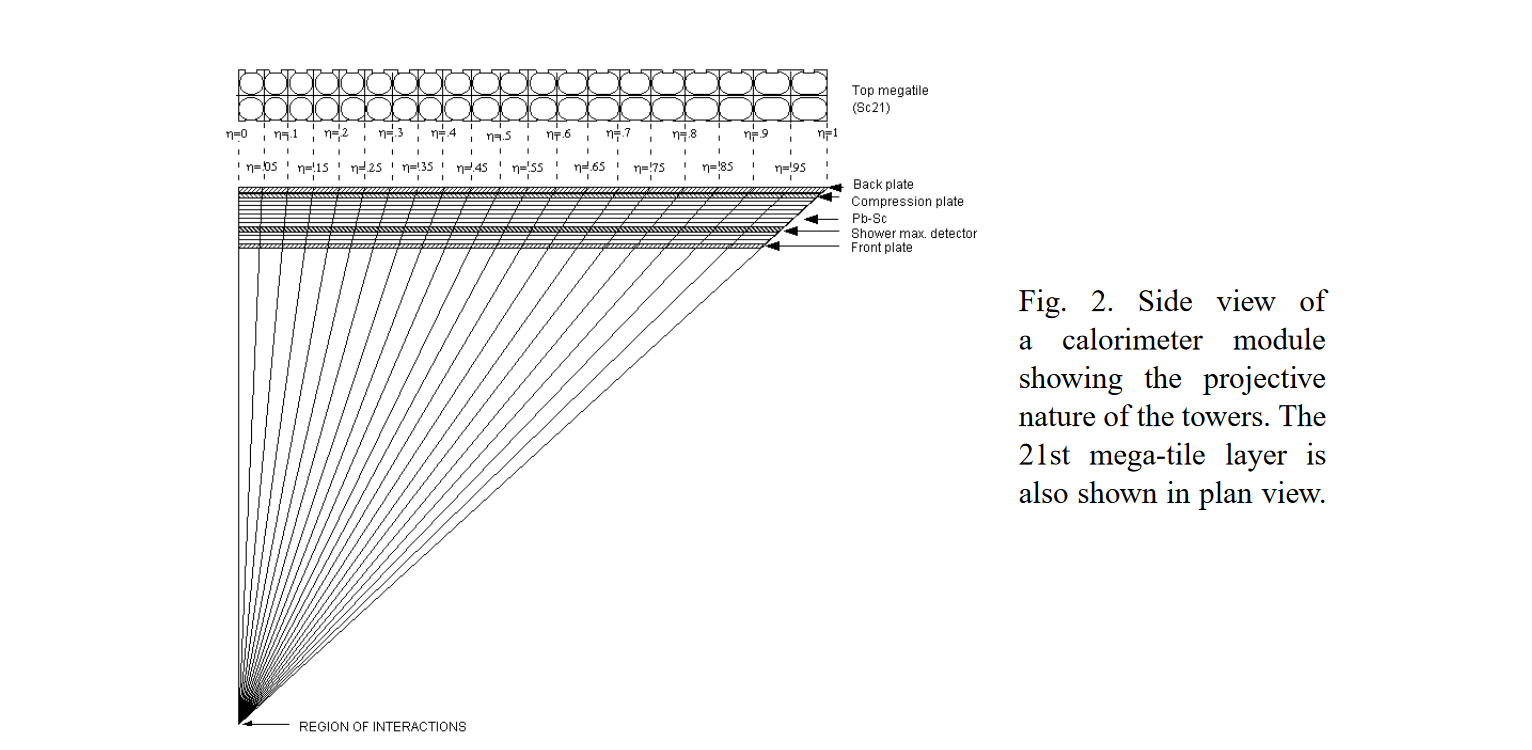
\includegraphics[width=7.5cm]{STAR_Detectors/BEMC_side_view} }}%
    \qquad
    \subfloat[\centering Δομή Μολύβδου-Σπινθηριστή]{{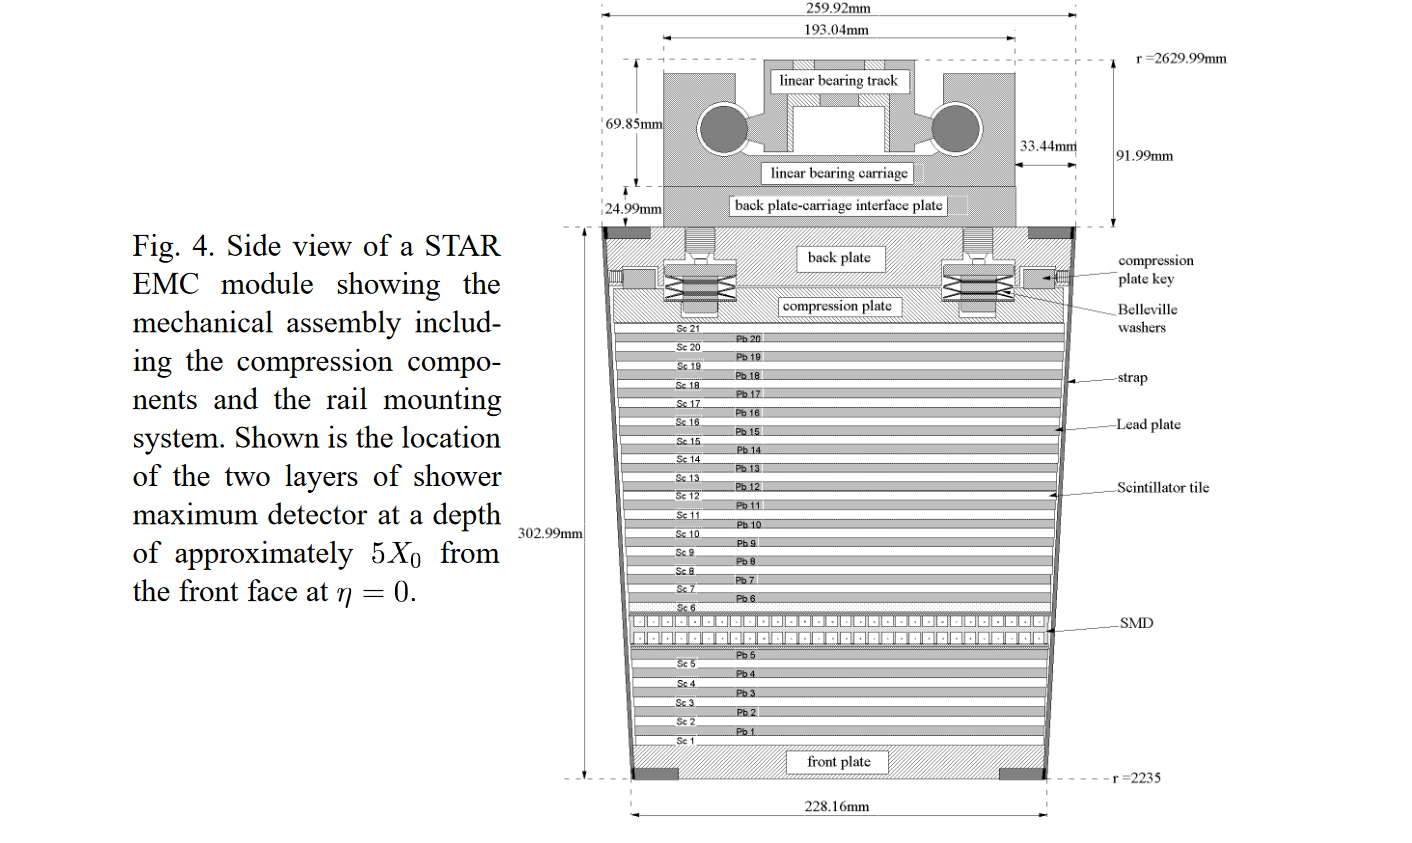
\includegraphics[width=7.5cm]{STAR_Detectors/BEMC_side_view2} }}%
    \caption{Πλευρικές όψεις του ΒΕΜC}
    \label{fig3.12}%
\end{figure}

	Τα 21 στρώματα σπινθηριστή του κάθε στρώματος είναι σε μορφή 40 ορθογωνίων παραλληλεπιπέδων εκ των οποίων τα 2 καλύπτουν γωνία $\phi$ και τα 20 $\eta$ όπως φαίνεται στην Εικόνα (\ref{fig3.12}b). Αυτοί είναι οπτικά απομονωμένοι και συνδέονται με μία οπτική ίνα, η οποία έχει καθορισμένη θέση εντός του στρώματος και μεταφέρει το σήμα στους φωτοπολλαπλασιαστές
	
	Τέλος, σε απόσταση περίπου 5.6$X_0$ από την αρχή του ανιχνευτή είναι εκεί όπου επιτυγχάνεται το μέγιστο της ενέργειας του καταιγισμού. Εκεί, διακόπτεται τοπικά η διαδοχή μολύβδού-σπινθηριστή και παρεμβάλλεται ένας αναλογικός ανιχνευτής αερίου (Shower Maximum Detector - SMD).
	Αυτός, επιτελεί τον σκοπό της βελτίωση της διαμήκους χωρικής διακριτικής ικανότητας που βοηθά στην ανακατσκευή των $\pi^0$, την ταυτοποίηση γ και e.
	
	O SMD αποτελείται από 50μm επιχρυσωμένα σύρματα βολφραμίου που είναι τοποθετημένα απέναντι από τμήματα καθόδου τα οποία ανιχνεύουν την αυξημένη συγκέντρωση φορτίου γύρω από τα σύρματα. To στοιχείο που βελτιώνει την απόδοσή του είναι πως υπάρχουν αντικριστά δύο επίπεδα από ανόδους-καθόδους, ένα πιό κοντά στην δέσμη και ένα πιό μακριά.
	